\section{Convolutional Neural Networks}
\label{sec:intro}

CNNs are a strong architecture for computer vision tasks. We are going to explore its performance on image classification.

%-------------------------------------------------------------------------
\subsection{CNN architecture}
We desinged our CNN with
\begin{itemize}
	\item 4 convolutional layers with ReLU and Maxpooling
	\item 4 fully connected layers with drop-out and ReLU
	\item Residual connections to every one layers
	\item Use CrossEntropy as a loss function for optimization
	\item The size of convolutional filter size 3
\end{itemize}
In addition, the input of our CNN is resized to 128*128 as Caltech101 dataset has image sizes 100 to 300. Detailed architecture including the dimension of channels are shown in \cref{fig:cnn_arch}. We tried to choose simplest yet high-performance model. Reasons for our choice will be introduced later.
\begin{figure}[htbp]
	\centering
	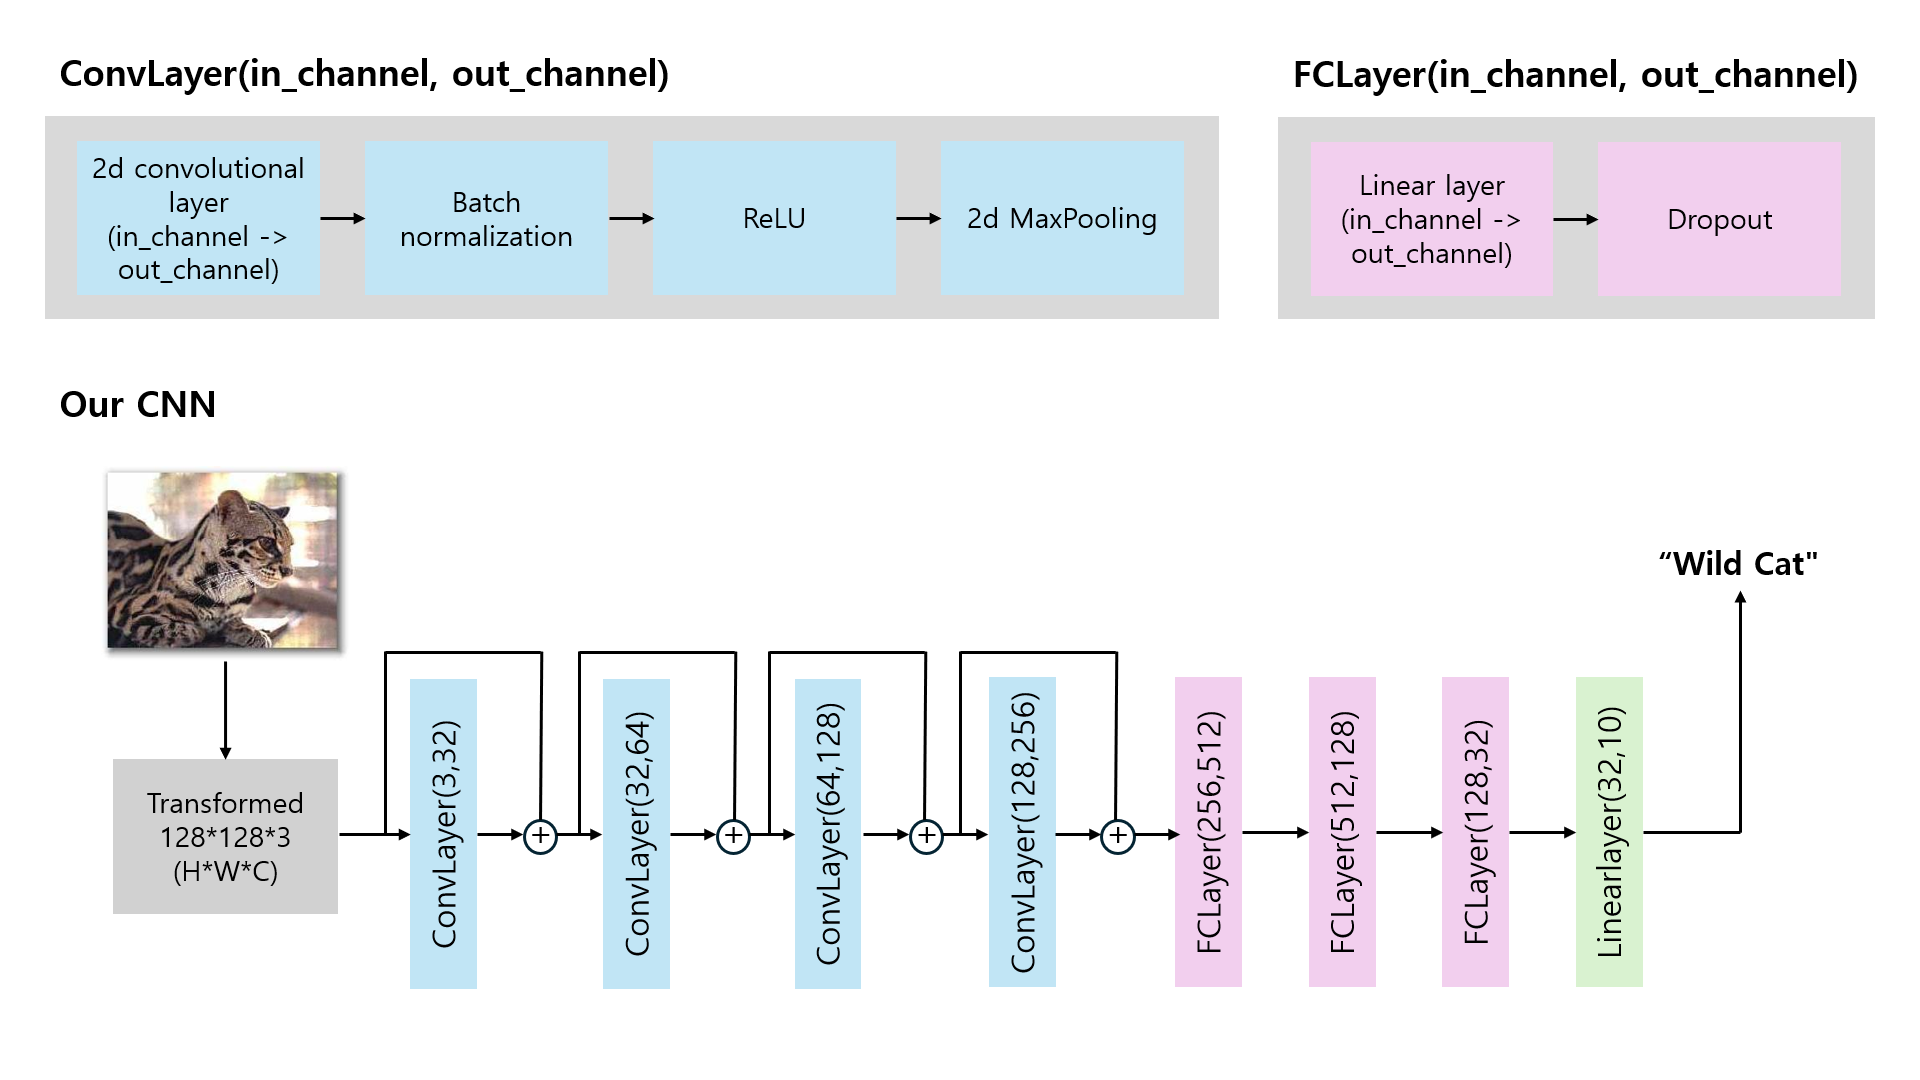
\includegraphics[width=0.7\linewidth]{image/q4-1-arch.png}
	\caption{Our CNN architecture}
	\label{fig:cnn_arch}
\end{figure}

\subsection{Changing architecture}
First, layers. We changed the number of layers from 3 to 5. As shown in \cref{fig:q4-2-layers}, the test accuracy is highest with 4 layers. It may because, when CNN has 3 layers, it is not enough to extract useful features from images and when it has 5, it may occur over-fitting due to the gradient vanishing. Hence, we conclude that 4 layers are the best choice for the performance.

Next, we changed the size of kernel to 3, 5, and 7. As \cref{fig:q4-2-kernel} shows, the accuracy is highest when the kernel size is 3 and it decreases as the kernel size increases. When the kernel size is small, it is adequate to capture the details of images and when the size is big, it is good to perceive the global scene. However, as our image has 128*128 size, which is small, kernel size 3 is enough to extract useful feature of the image. other sizes are too big to recognize the features corresponding the image label.

Lastly, we conduct the experiments on residual connection between layers. There are three cases: no connection between layers, connect every 2 layers, connect every one layers. Since we have total 4 layers, the number of connections are 0, 2, and 4 for each. The test accuracy are shown in \cref{fig:q4-2-connection}. It increases as the number of connection increases. It is because,  using residual connection, CNN does not lose the information from initial layers thus it can learn more general information about images and its label.

\begin{figure}[htbp]
	\centering
	\begin{subfigure}[t]{0.3\linewidth}
		\centering
		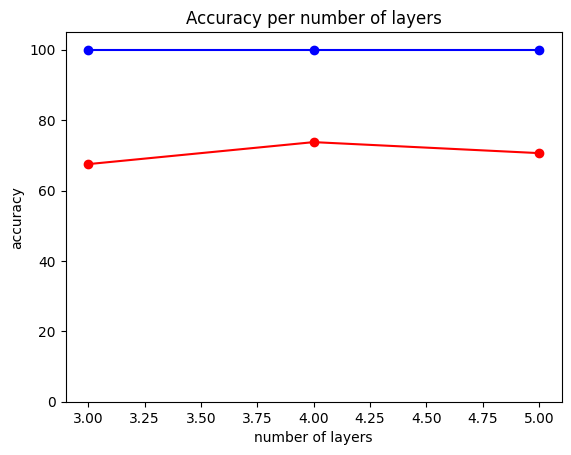
\includegraphics[width=\linewidth]{image/q4-2-layers.png}
		\caption{Accuracy according to layers}
		\label{fig:q4-2-layers}
	\end{subfigure}	
    \hfill
	\begin{subfigure}[t]{0.3\linewidth}
		\centering
		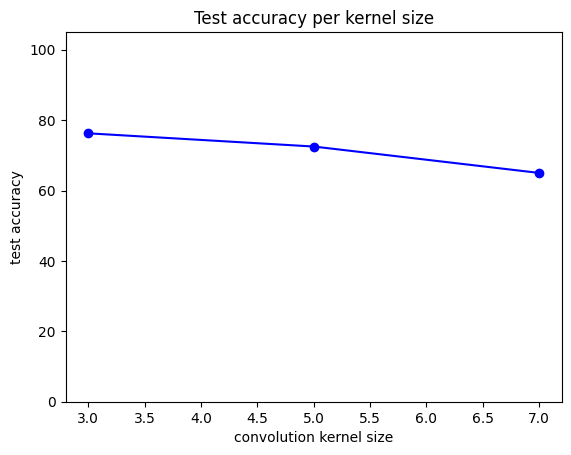
\includegraphics[width=\linewidth]{image/q4-2-kernel.png}
		\caption{Accuracy according to kernel size}
		\label{fig:q4-2-kernel}
	\end{subfigure}%
    \hfill
	\begin{subfigure}[t]{0.3\linewidth}
		\centering
		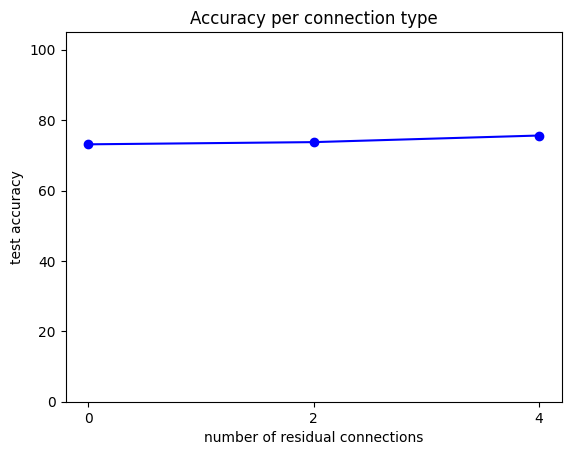
\includegraphics[width=\linewidth]{image/q4-2-connection.png}
		\caption{Accuracy according to connections}
		\label{fig:q4-2-connection}
	\end{subfigure}

	\caption{impact of changing architecture of CNNs}
	\label{fig:cnn_architecture}
\end{figure}

\subsection{Layer normalization}
To explore the effect of the layer normalization method, we test our model using 4 different methods: batch, layer, instance, and group.

The accuracies per batch number for each method are shown in \cref{fig:normalization}. We can check that batch normalization is greatly affected by the size of the batch, while the other methods show consistent accuracy regardless of the size of the batch.

For batch normalization, the larger the batch size, the higher the accuracy. This is because larger batches are more robust to noise since they can closely estimate the true distribution of the training data. However, too large batch is inaccurate because we can not expect generalization effect due to the randomness of batch training. These are the reason why batch size 16 has the largest accuracy.

In image classification, it is important to catch the difference between feature distribution of within and between classes. Using batch normalization, we can consider class distribution since the normalization is performed on a batch basis. However, other methods only do normalization within a single image, the information related to class statistics is weakened. Hence, their accuracy becomes lower than using batch normalization.

\begin{figure}
	\centering
	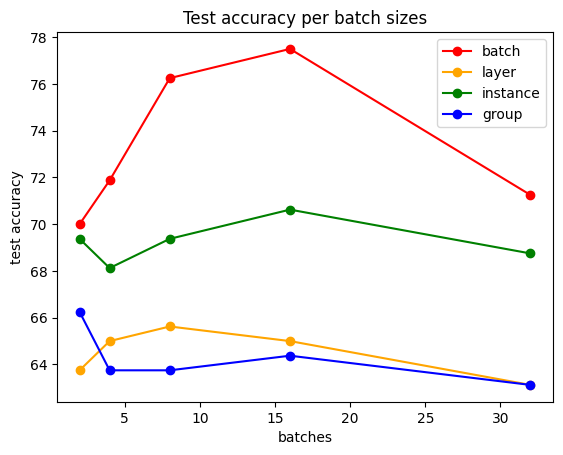
\includegraphics[width=0.4\linewidth]{image/q4-3.png}
	\caption{Accuracy according to normalization types}
	\label{fig:normalization}
\end{figure}

\subsection{Generalization}
There are many method for Generalization of CNN. In this section, we are going to check the impact of drop-out and L2-regularization on weights(which is in Deep\_Learning\_intro Lecture Note pg.84). We test our basic model which has drop-out, the model without drop-out, and the model with L2-regularization on weights. Results are shown in \cref{table:generalization}. The model without drop-out has the lowest accuracy and the model with L2-regularization has the highest accuracy. This is because, drop-out randomly deactivate some neurons, so it helps model to avoid overfitting and be good at generalization. And L2-regularization helps model to avoid overfitting by regulate the size of weights.
Hence, it is natural result that the model with both drop-out and L2-regularization has the best performance.

\begin{table}
	\centering
	\setlength{\tabcolsep}{6pt}
	\renewcommand{\arraystretch}{1.5}
	\resizebox{0.5\linewidth}{!}{
		\begin{tabular}{|c||c|}
		\hline
		& accuracy  \\ \hline\hline
		original & 75.625  \\ \hline
		without dropout & 68.125  \\ \hline
		with L2-regularization term & 76.250  \\ \hline
		\end{tabular}
	}
    \caption{Impact of generalization}
	\label{table:generalization}
\end{table}
	

\subsection{Loss function}
We use CrossEntropy, which is based on softmax function, as a loss function as usual. And compare it with SquaredHinge loss.

Using CrossEntropy for the loss function, we get 73.75\% accuracy while we get 80.00\% accuracy with SquaredHinge loss, which is higher. This is because, as CrossEntropy is based on probability distribution and SquaredHinge loss is based on the margin between expected and real classes, SquaredHinge is better since our dataset is small. (which has only 10 classes) In more detail, because the dataset is small, it is hard to estimate an accurate probability distribution due to the law of large numbers. Hence, it is better to use direct borders and margins between classes. Despite this reason, we adopted CrossEntropy as a basic loss function as it is widely used.

\subsection{Compressing CNN}
We conduct an experiment on compressing layers of CNN using truncated SVD. Our model has 4 fc layers with rank 512, 128, 32, 10, and we compress first two layers with 100(original), 75, 50, 25 percent each because last two layers are too small to compress. The result are shown in \cref{fig:cnn_svd}. Test accuracy and time are both decreased as layers are more compressed. It is because, as weight matrix of layers become compressed, there remain less computation to get the result, but it causes more data loss.

\begin{figure}
	\centering
	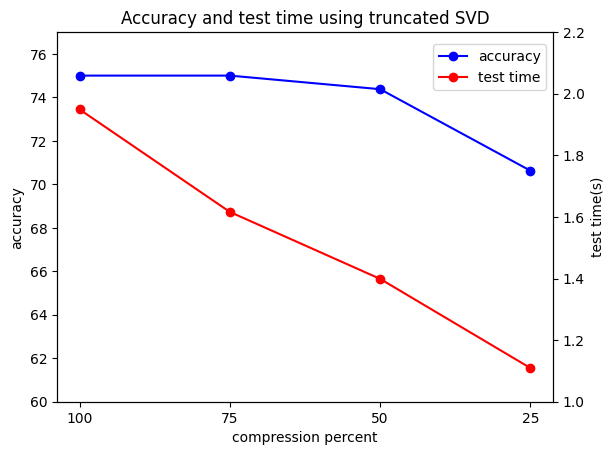
\includegraphics[width=0.4\linewidth]{image/q4-6-svd.png}
	\caption{Accuracy and test time using truncated SVD}
	\label{fig:cnn_svd}
\end{figure}

\subsection{Changing parameters}
We observe the influence of main hyper-parameters by experiments. We changed 3 parameters from base model: learning rate, batch size, and the number of epochs.

\cref{fig:q4-7-lr-train} and \cref{fig:q4-7-lr} indicates the result of varying learning rate. We changed learning rate to 0.00001, 0.0001, 0.0005, and 0.005. When the learning rate is 0.00001, the model doesn't converge sufficiently since it is too small to reach the local minimum of loss during the given epochs. And when the learning rate is 0.0005 and 0.001, it vibrates too much until it reaches the convergence point. More specifically, amplitude of 0.001 is larger than 0.0005. This is because, the amount of moving is too big, so, the model oscillates near the local minimum largely. Therefore, we decided that learning rate = 0.0001 is the best for our model. Regarding the accuracy, the accuracy is higher when the learning rate is 0.0001 and less than this when the learning rate is smaller or bigger than 0.0001. It is because, if the learning rate is too small, it can not converge in the training time sufficiently and if the it is too big, it might pass through optimization point.

For the batch size, we trained our model with batch size from $2^1$ to $2^6$. And we get the highest accuracy when the batch size is 16.(\cref{fig:q4-7-batch}) This is because, with small batch, the model learns the feature distribution from small amount of data, so, the train result can be largely different from whole data distribution. Conversely, if the batch size is too big, it is vulnerable at generalization since we can not expect generalization effect from increasing randomness of training as smaller batch. Generally, batch size 32 is not big enough to cause the over-fitting but considering that size of our training dataset is 150, 32 is quite large number. Therefore, it is reasonable that batch size 16 is enough to get enough meaningful features while avoiding over-fitting. In addition, test time decreases using bigger batch because of parallel computing on GPU in batch units. In general, we can conclude that there is a trade off between accuracy and test time on batch size.

Lastly, for the number of epochs, we use 75, 100, 125, 200 epochs and compared the result. Results are shown in \cref{fig:q4-7-epoch}. The accuracy is the highest with 100 epochs because when the number of epoch is not enough, it can cause under-fitting while large amount of epochs can cause over-fitting.

\begin{figure}
	\centering
	\begin{subfigure}{0.23\linewidth}
		\centering
		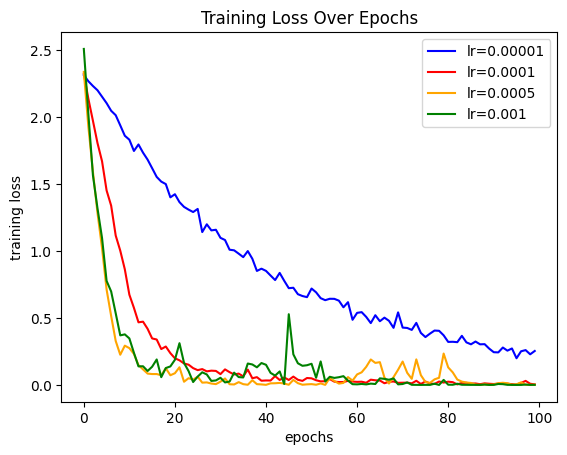
\includegraphics[width=\linewidth]{image/q4-7-lr-train.png}
		\caption{Learning rate training losses}
		\label{fig:q4-7-lr-train}
	\end{subfigure}%
	\hfill
	\begin{subfigure}{0.23\linewidth}
		\centering
		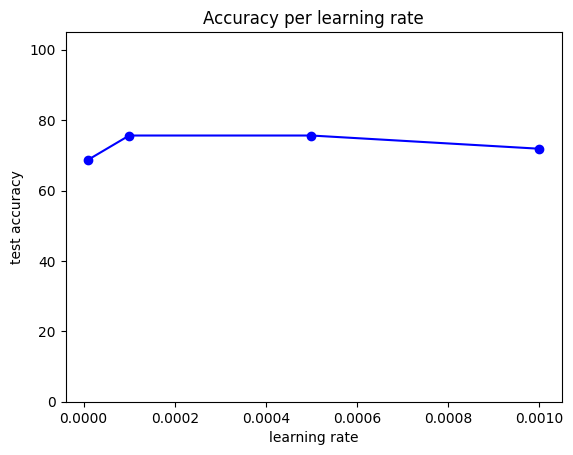
\includegraphics[width=\linewidth]{image/q4-7-lr.png}
		\caption{Learning rate accuracy}
		\label{fig:q4-7-lr}
	\end{subfigure}
	\hfill
	\begin{subfigure}{0.23\linewidth}
		\centering
		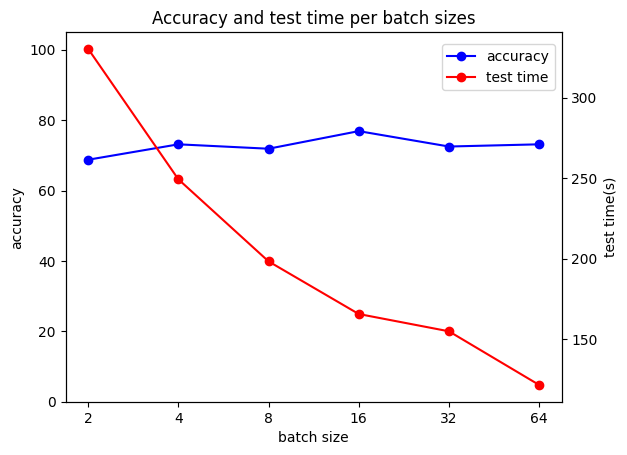
\includegraphics[width=\linewidth]{image/q4-7-batch.png}
		\caption{Batch size accuracy}
		\label{fig:q4-7-batch}
	\end{subfigure}
	\hfill
	\begin{subfigure}{0.23\linewidth}
		\centering
		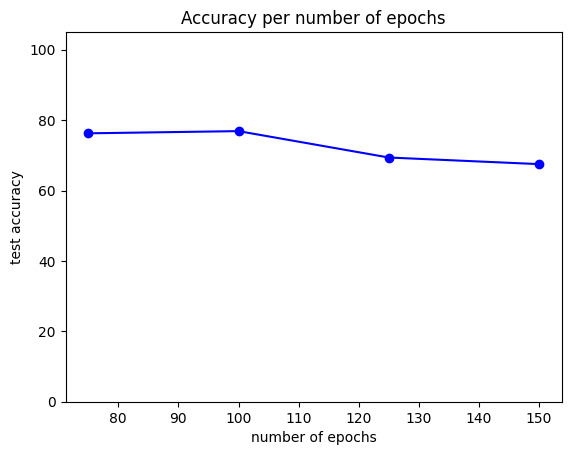
\includegraphics[width=\linewidth]{image/q4-7-epoch.png}
		\caption{Epoch accuracy}
		\label{fig:q4-7-epoch}
	\end{subfigure}
	\caption{Changing hyper-parameters of CNN}
	\label{fig:q2}
\end{figure}

\subsection{Pre-trained model}
In this section, we compare training methods: fine-tuning pre-trained model and training from scratch from random initialization. Since our CNN does not have pre-trained version, we used pre-trained ResNet model(microsoft/resnet-50, trained with ImageNet) and custom it with Caltech101 dataset. Due to the time limit, we only train it with 10 epochs. When we use pre-trained weights and fine-tuned them, we get 99.33\% accuracy. And training from scratch with random initialization, we get 21.33\% accuracy which is lower than before. Based on this result, with the limited amount of time and resources, it is much better to use pre-trained model to get high performance. It is because, since we used pre-trained model with same task(image classification), trained weight is specialized for image classification even with different dataset. Therefore, fine-tuning using a custom dataset can achieve higher accuracy with fewer resources than training from scratch.

\subsection{Comparison with other methods}
Considering that our CNN have accuracy about 75\%, it is much better model than RF classifier in Q2 and Q3 as shown in \cref{table:accuracy}. This is because CNN can do end-to-end learning from feature extraction to classification, unlike Q2 and Q3's model. In other words, k-means or random forest vocabulary followed by random forest classification does not allow end-to-end learning, making it difficult to determine whether the vector quantisation result includes beneficial features for classification. However, CNN can automatically learn various meaningful representations directly from raw data.

\begin{table}[htbp]
	\centering
	\setlength{\tabcolsep}{6pt} % Adjust column spacing
	\renewcommand{\arraystretch}{1.5} % Adjust row height
	\resizebox{0.5\textwidth}{!}{ % Scale table to fit text width
		\begin{tabular}{|c||c|c|}
			\hline
			& Train Accuracy (\%) & Test Accuracy (\%) \\ \hline\hline\
			K-means Codebook - RF Classifier & 99.50 & 68.5   \\ \hline
			RF Codebook - RF Classifier & 97.80 & 60.67  \\ \hline
			CNN & 100.00 & 75.625  \\ \hline
		\end{tabular}
	}
	\caption{Accuracy of Models}
	\label{table:accuracy}
\end{table}